%!TEX root = main.tex
\chapter{Physical Modeling}
\label{Karplus}

\begin{figure}[h]
  \begin{center}
    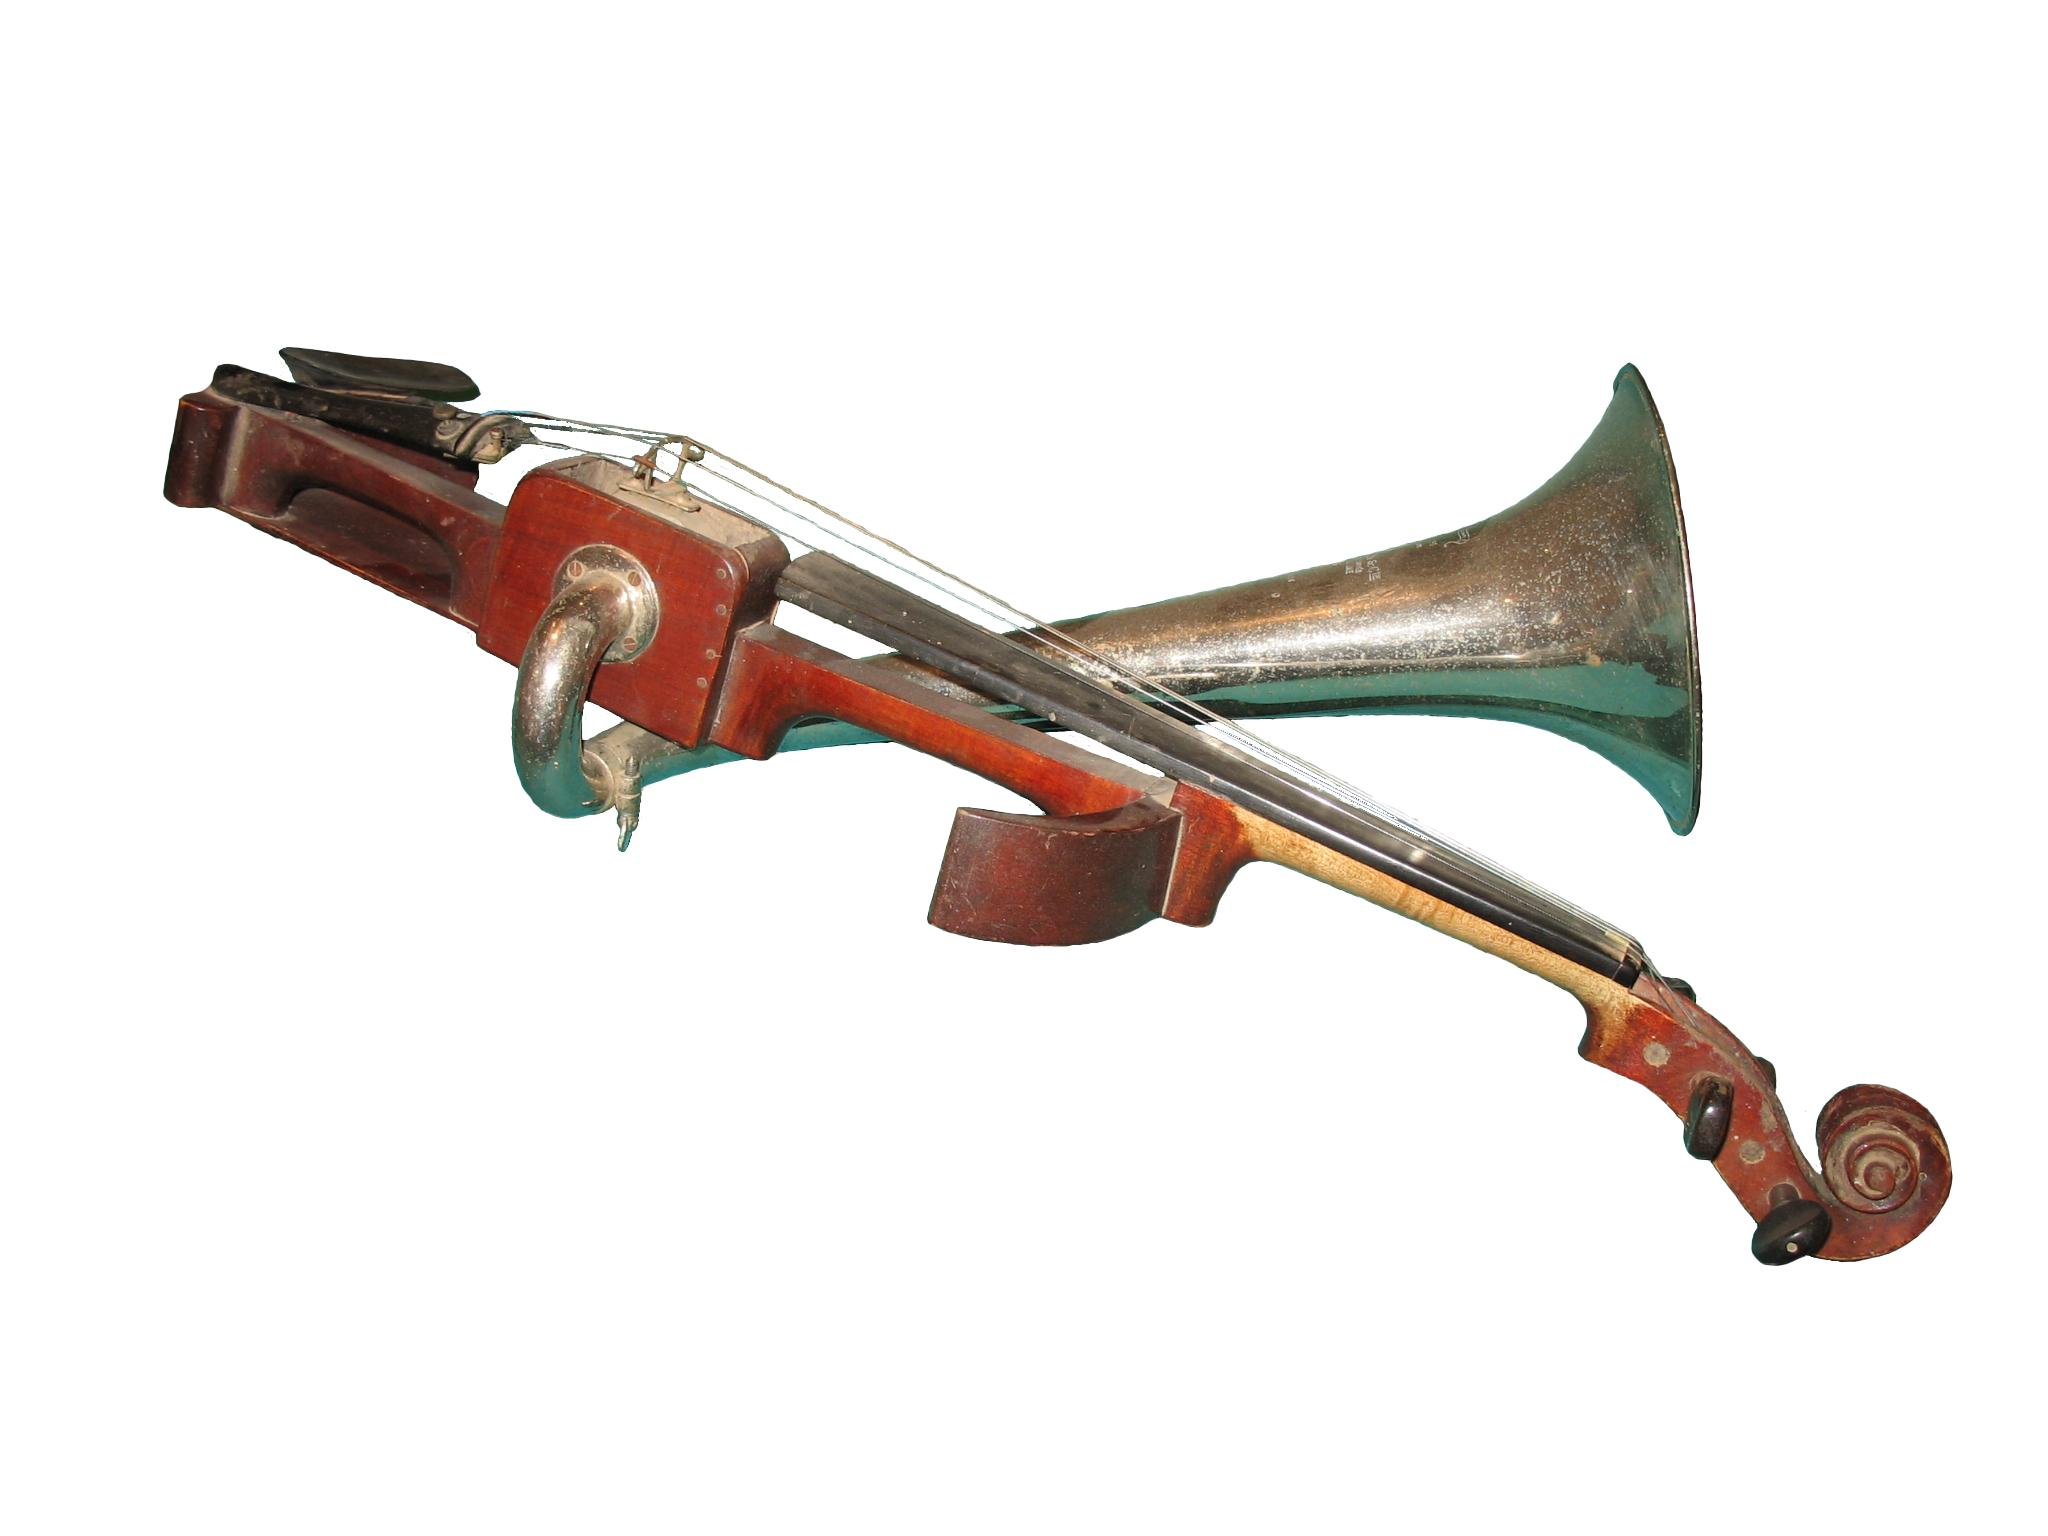
\includegraphics[width = 14cm]{img/strohgeige.jpg}
    \caption{Die Strohgeige, ein eigentuemliches Saiteninstrument}
    \label{fig:metering}
  \end{center}
\end{figure}


\section{References}

\begin{itemize}
  \item \cite{bilbao_numerical_2009}
  \item \cite{smith_physical_2010}
  \item \cite{cook_real_2002}
\end{itemize}


% Karplus strong und PM,\\
% schwingungssysteme,\\
% simulation..

% Ableton Live: donner,\\
% rechtfertigung: Computerspiele, etc.\\
% (Wellen-)Experiment.\\
% Geschichte: Bernoulli und D'Alembert\\
% Wellengleichung
% Karplus Strong (bauen, geschichte erzählen)
% (Pause)
% Waveguide, Scattering Junctions erwähnen undje nach interesse behandeln. Kelly und Lochbaum modell.
% Kaffeehäferl synthetisieren. (Praat, reson)



\section{Further Information}

\begin{itemize}
  \item \link{https://www.youtube.com/watch?v=Li6OEMCtQ9k}{Wave Equation}
  \item \link{https://www.youtube.com/watch?v=dUcNzPhZdwk}{Julius O. Smith about Physical Modeling in Stanford}
  \item \link{http://www.fon.hum.uva.nl/praat/}{Praat audio analysis}
\end{itemize}



\section{Overview}


\begin{enumerate}
	\item motivation: games, and efficient realistic sound generation
	\item PM: erklärung
	\item Karplus-Strong
	\item Schulübung: sounddesign challenge in pd.

\end{enumerate}

\section{Theory: Oscillating Systems}


Wave equation, infinite one-dimensional string:
\begin{equation}
	c^2 \cdot \frac{\delta^2 f}{\delta x^2} = \frac{\delta ^2 f}{\delta t ^2}
\end{equation}

Visualization:

\begin{figure}[H]
  \begin{center}
    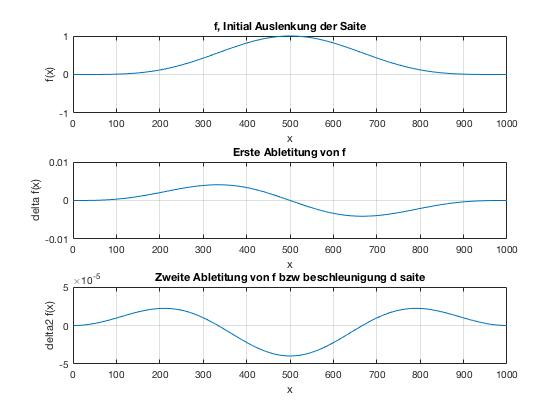
\includegraphics[width = 14cm]{img/wellengleichungVis.png}
    \caption{Visualisierung der Wellengleichung}
    \label{fig:wellengleichung}
  \end{center}
\end{figure}




Two possible solutions for the differential equation:
\begin{itemize}
	\item Bernoulli = ca. fourier, spectral, summe von sinus schwingungen.
	\item D'Alembert = ca. Physical modeling, zwei funktionen die entlang der saite reisen (in entgegengesetzte richtung).
\end{itemize}

Bernoulli:
\begin{equation}
  y(t,x) = \sum^{\infty}_{k=0} A_k sin(k\pi x/L)cos(k\pi \nu t)
\end{equation}
(Displacement length $L$, vibrating string at time $t$ at position $x$, frequency $\nu$)

\begin{equation}
y(x, t) = y ^+ \Bigg(t - \frac{x}{c}\Bigg) + y^- \Bigg(t + \frac{x}{c} \Bigg)
\end{equation}

\section{Karplus Strong Synthesis}
% D'Alembert sagt also, es gäbe zwei wellen, die in zwei richtungen entlang der saite reisen, die Lässt sich einfach simulieren, mittels zwei in einander geschalteten delays.
So D'Alembert says, there are two waves, one traveling to the right and one traveling to the left. Their superposition is what makes up the actual wave along a string. \\
Observing a string more closely, we find that a wave gets inverted at its borders and travels back.
All this can easily be simulated in a computer, see Figure~\ref{fig:string}.


  \begin{figure}[htb]
  \centering
  \label{fig:string}

  % \resizebox{10cm}{!}{%
  \begin{tikzpicture}[auto, thick, node distance=2.3cm, >=triangle 45]

  \draw node at (5,0) [block] (del1) {\Large$\ \ \ \ \ \ \ \ z^{-m}\ \ \ \ \ \ \ \ $};
  \draw node at (5,-3) [block] (del2) {\Large$\ \ \ \ \ \ \ \ z^{-m}\ \ \ \ \ \ \ \ $};
  \draw node at (0, -1.5) [mult] (m1) {\Large$-1$};
  \draw node at (10, -1.5) [mult] (m2) {\Large$-1$};

  \draw[->] (del1) -| node {}(m2);
  \draw[->] (m2) |- node {}(del2);
  \draw[->] (del2) -| node {}(m1);
  \draw[->] (m1) |- node {}(del1);

  \end{tikzpicture}
  \caption{general idea of Waveguide synthesis/Karplus-Strong Model.}
\end{figure}

The model in Figure~\ref{fig:string} is a rather theoretical one\footnote{You might notice that there are no inputs and no outputs. This structure is theoretical for us, since we do not talk about something called the \textit{Wave Digital Filter}(WDF). When talking about WDFs we find similar structures since they are strongly inspired by physics. Since in physics we always have a force and another force counteracting the first one we always have left and right traveling energy.}. But it leads us to a more useful implementation. Since all elements in Figure~\ref{fig:string} are LTI, we can rearrange them in any order. Multiplying a signal times $-1$ two times is the same as doing nothing. And two delays of length $m$ are equivalent to one delay of length $2m$.\\
So we arrive at a simple delay with feedback. To simulate energy loss we need to attenuate the feedback signal and to simulate frequency dependent loss, we can use a lowpass filter inside the feedback loop. After all this, we arrive at Figure~\ref{fig:string2}.

\begin{figure}[h!]
  \centering

  \label{fig:string2}

  \begin{tikzpicture}[auto, thick, node distance=2.3cm, >=triangle 45]

  \draw node at (0,0) [input] (excitation) {};
  \draw node [sum, right of=excitation, node distance = 2.cm] (sum1) {\Large$+$};
  \draw node [block, right of=sum1, node distance = 2cm] (delay) {\Large$z^{-m}$};
  \draw node [block, below of=delay, node distance = 2cm] (loss) {\Large$G(z)$};
  \draw node at (6.,-0.001) {\textbullet};

  \draw node [output, right of=delay,node distance = 3cm] (out) {};
  \draw[->] (excitation) -- node {\Large$x[n]$}(sum1);
  \draw[->] (sum1) -- node {}(delay);
  \draw[->] (loss.west) -| node {}(sum1.south);

  \draw[->] (6., -0.001) |- node {}(loss.east);


  \draw[->] (delay) -- node {\Large$y[n]$}(out);

  \end{tikzpicture}
  \caption{single string, $G(z)$ a lowpass, \glqq{}Loss Filter\grqq{}}
\end{figure}

\section{Practical Karplus-Strong}
\begin{figure}[H]
	\begin{center}
		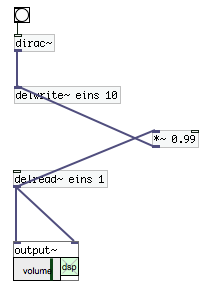
\includegraphics[scale = 1.]{img/karplusSimple.png}
		\caption{Basic setup}
		\label{fig:karplusBasic}
	\end{center}
\end{figure}


\section{Modal Synthesis with Bandpass filters}


\section{Schulübung, Sounddesign challenge}

zB:
\begin{itemize}
	\item Vokal
	\item E-gitarre
	\item beliebiges Physikalisches object

\end{itemize}

% \section{Hausuebung}
% Andy Farnell, \href{http://aspress.co.uk/ds/pdf/pd_intro.pdf}{pd intro} chater 7, lesen

